\chapter{Metodología}
\label{ch:Methodology}

% [Integrado desde drafts/ch4_*.tex el 2026-07-20. Pase 2 (redaccion desde wiki/).]
% Tabla de parametros numericos de la Sec. 4.6.4 integrada el 2026-07-22
% (tables/tabla_4_6_4.tex, generada por scripts/make_table_4_6_4.py).

Este capítulo convierte la pregunta de investigación en un método concreto: detalla cómo se construye el estudio comparativo y con qué criterios se ejecuta, de modo que cada uno de los seis objetivos específicos (Sección~\ref{sec:objetivos}) se materialice en un componente verificable.

La exposición sigue el orden lógico en que se encadenan esos objetivos. La
Sección~\ref{sec:modelo_numerico} construye el \emph{simulador de la cavidad} a partir
de la ecuación maestra de Haus (sus variantes activa y pasiva, su integración
numérica y su verificación), que actúa como entorno de evaluación (primer objetivo).
Sobre él, la Sección~\ref{sec:formulacion_problema} \emph{formula el problema de
optimización}, fijando las variables de decisión, sus rangos y restricciones, y la
función de mérito (segundo objetivo). Las tres secciones siguientes especifican la
implementación de cada estrategia sobre ese problema común: el algoritmo genético que
sirve de línea base (Sección~\ref{sec:ga_impl}; tercer objetivo), la red neuronal
acoplada como modelo sustituto (Sección~\ref{sec:nnga_impl}; cuarto objetivo) y la
optimización por enjambre de partículas (Sección~\ref{sec:pso_impl}; quinto objetivo).
Finalmente, la Sección~\ref{sec:diseno_experimental} define el \emph{protocolo
comparativo} (las métricas, las condiciones que se mantienen idénticas, el control de
la aleatoriedad y las decisiones de reproducibilidad) con el que se contrastan los
tres métodos (sexto objetivo).

Dos hilos recorren todo el capítulo y conviene anticiparlos. El primero es que el
estudio se realiza enteramente en \emph{simulación}: la cavidad no se monta, se
integra numéricamente, y ese simulador es a la vez el objeto que reproduce la física
y el entorno que evalúa a los optimizadores. El segundo es el principio que ordena el
diseño experimental: mantener fijo todo lo que no es el algoritmo (el mismo láser, el
mismo espacio de parámetros y la misma función de mérito) y variarlo únicamente a él,
sobre las dos modalidades de bloqueo de modos, para que las diferencias de desempeño
que se observen puedan atribuirse a la mecánica de búsqueda y no a las
particularidades del problema. Es esa disciplina comparativa, más que cualquier
método individual, lo que constituye el aporte metodológico de la tesis
(Sección~\ref{sec:aporte}).


% ============================================================
%  Seccion 4.1 -- Modelo numerico de la cavidad (OE1)
% ============================================================

\section{Modelo numérico de la cavidad}
\label{sec:modelo_numerico}

El estudio necesita un modelo numérico de la cavidad láser que reproduzca los regímenes de operación conocidos y sirva de entorno de evaluación para los algoritmos; construirlo es el primer objetivo específico (Sección~\ref{sec:objetivos}). Esta sección parte de la ecuación maestra de Haus (Sección~\ref{sec:haus}), la especializa a los dos regímenes que compara el estudio (bloqueo de modos activo y pasivo), fija el método de integración numérica, define el criterio de estado estacionario y los observables que se extraen del pulso, y verifica el simulador contra las soluciones analíticas conocidas. El resultado es la caja negra $\mathbf{p}\mapsto F(\mathbf{p})$ que la
Sección~\ref{sec:formulacion_problema} convertirá en un problema de optimización
bien planteado.

\subsection{La ecuación maestra de Haus como entorno de evaluación}
\label{sec:sim_entorno}

El modelo de la cavidad es la ecuación maestra de Haus en su forma general
\eqref{eq:haus_general}, que reúne en una sola expresión la amplificación con
filtrado de ganancia, las pérdidas, la dispersión de la velocidad de grupo, la
automodulación de fase y el mecanismo de bloqueo de modos:
%
\begin{equation}
    T_R\,\frac{\partial A}{\partial T}
    = \Bigl[\,(g-l)
      + \bigl(D_g + iD\bigr)\frac{\partial^2}{\partial t^2}
            - i\,\delta\,|A|^2
      + \Delta_{\mathrm{ML}} \,\Bigr] A .
    \label{eq:sim_maestra}
\end{equation}
%
% [REV-2026-11-24] el código conserva la convención conjugada; se documenta la equivalencia
El simulador implementa la ecuación conjugada de~\eqref{eq:sim_maestra}, con
$+i\delta|A|^2$ y dispersión anómala para $D>0$. Ambas formas son equivalentes por la
sustitución $A\to A^{*}$, $D\to-D$, y los observables, que dependen de $|A|^2$, no
cambian; los valores de $D$ que se reportan en este texto siguen la convención de la
ecuación~\eqref{eq:sim_maestra}, es decir, el signo opuesto al de los archivos de
configuración y de resultados.
La ecuación~\eqref{eq:sim_maestra} descansa sobre las dos escalas temporales
propias del formalismo de Haus \cite{Haus2000,Kaertner2020}: el \emph{tiempo local}
$t$, que resuelve el perfil de la envolvente $A$ dentro de una ventana mucho más
corta que el periodo de repetición, y el \emph{tiempo lento} $T$, que numera la
evolución de la envolvente de una vuelta a la siguiente en pasos del tiempo de ida y
vuelta $T_R$. Cada término del corchete es el efecto acumulado, por ronda, de un
elemento intracavitario, bajo la hipótesis de que ese efecto produce un cambio
pequeño en la envolvente por vuelta (Sección~\ref{sec:haus}).

Concebir la cavidad como \emph{entorno de evaluación} significa leer la
ecuación~\eqref{eq:sim_maestra} en clave de simulación. Los coeficientes
$\{g,\,l,\,D_g,\,D,\,\delta\}$ y los que parametrizan $\Delta_{\mathrm{ML}}$ son las
entradas: fijar sus valores equivale a fijar un punto $\mathbf{p}$ del espacio de
decisión \eqref{eq:vector_decision}. Integrar la ecuación en $T$ a partir de una
semilla inicial, hasta que la envolvente deja de cambiar de una vuelta a la
siguiente, produce la salida: el pulso estacionario del que se extraen los
observables (Sección~\ref{sec:sim_estacionario}). La condición de estacionariedad es
la que ya introdujo el marco teórico, esto es, que el pulso se reproduzca a sí mismo
salvo un desfase global por ronda, $A(T,t)=A(t)\,e^{i\phi_0 T/T_R}$
\eqref{eq:haus_estacionario}. El simulador no es, por tanto, más que el operador que
lleva un vector de parámetros al pulso que la cavidad emitiría en régimen
permanente; su relación con las variables no se conoce en forma cerrada y solo se
accede a ella evaluándola, el rasgo de caja negra que caracteriza al problema
(Sección~\ref{sec:estructura_espacio}).

\subsection{Variante de bloqueo de modos activo}
\label{sec:sim_activo}

En el régimen activo, el mecanismo de bloqueo de modos es un modulador de amplitud
externo que impone una pérdida periódica sincronizada con la cavidad,
$\Delta_{\mathrm{ML}}^{\text{act}}A=-M(1-\cos\omega_m t)\,A$
\eqref{eq:op_modulador}, con $M$ la profundidad de modulación y $\omega_m$ su
frecuencia, igual a la de repetición. Sustituido en~\eqref{eq:sim_maestra}, define
el modelo del brazo activo del simulador:
%
\begin{equation}
    T_R\,\frac{\partial A}{\partial T}
    = \Bigl[\,(g-l)
      + \bigl(D_g + iD\bigr)\frac{\partial^2}{\partial t^2}
      - i\,\delta\,|A|^2
      - M\bigl(1-\cos\omega_m t\bigr) \,\Bigr] A .
    \label{eq:sim_activo}
\end{equation}
%
El vector de decisión de este régimen agrupa, por tanto, los coeficientes
$\{g,\,l,\,D_g,\,D,\,\delta,\,M,\,\omega_m\}$. Conviene distinguir dos modos de uso
del modelo~\eqref{eq:sim_activo}, que se corresponden con las dos especializaciones
del marco teórico. Si se anulan la dispersión y la no linealidad netas
($D=\delta=0$), la ecuación se reduce al límite de Kuizenga--Siegman
\eqref{eq:haus_activo_base}, cuyo pulso estacionario es una gaussiana cuya anchura
fija el balance entre la dispersión de ganancia $D_g$, que ensancha, y la curvatura
del modulador $M_s\equiv M\omega_m^2/2$, que estrecha
(Sección~\ref{sec:kuizenga_siegman}). Si, en cambio, se conservan una dispersión
anómala y una automodulación de fase suficientes, el conformado por solitón se
superpone a la modulación y da lugar a pulsos apreciablemente más cortos, en el
régimen de bloqueo de modos activo con formación de solitón
(Sección~\ref{sec:ml_activo_soliton}) \cite{Kaertner2020}. El simulador contempla
ambos modos: el primero por su solución analítica cerrada, que sirve de referencia
de verificación (Sección~\ref{sec:sim_verificacion}); el segundo por ser el
físicamente pertinente cuando se busca el pulso más corto. La estructura más
determinista y de menor dimensión efectiva de este régimen es, además, uno de los
motivos por los que la tesis lo incorpora junto al pasivo, habitualmente más
explorado (Sección~\ref{sec:aporte}).

\subsection{Variante de bloqueo de modos pasivo}
\label{sec:sim_pasivo}

En el régimen pasivo, el mecanismo de bloqueo de modos es un absorbente saturable
que atenúa selectivamente las componentes de baja intensidad,
$\Delta_{\mathrm{ML}}^{\text{pas}}A=-q(|A|^2)\,A$ \eqref{eq:op_absorbente}. A
diferencia del modulador externo, el absorbente es \emph{gobernado por el propio
pulso}: la ventana de baja pérdida se estrecha con el pulso y lo sigue de forma
automática, lo que da acceso al régimen de femtosegundos donde el activo se detiene
en los picosegundos (Sección~\ref{sec:haus_pasivo}).

El comportamiento del absorbente depende de la relación entre su tiempo de
relajación $\tau_A$ y la duración del pulso $\tau_p$
(Sección~\ref{sec:absorbente_tipos}) \cite{Keller2022}. Cuando la recuperación es
mucho más rápida que el pulso ($\tau_A\ll\tau_p$), la absorción sigue
instantáneamente a la potencia y, en la aproximación de saturación débil que hace
tratable el modelo, se linealiza como
%
\begin{equation}
    q\!\left(|A|^2\right) \approx q_0 - \gamma\,|A|^2,
    \qquad \gamma \equiv \frac{q_0}{I_{\mathrm{sat},A}},
    \label{eq:sim_absorbente_rapido}
\end{equation}
%
donde $q_0$ es la pérdida no saturada e $I_{\mathrm{sat},A}$ la intensidad de
saturación \eqref{eq:op_absorbente_rapido}. Cuando la recuperación es mucho más
lenta que el pulso ($\tau_A\gg\tau_p$), en cambio, el absorbente se satura con la
energía integrada del pulso y su pérdida deja de depender de la forma instantánea,
lo que exige acoplar una ecuación de tasa propia y, típicamente, la saturación
dinámica de la ganancia \cite{Keller2022,Kaertner2020}.

\paragraph{Decisión de modelado.}
El simulador adopta como modelo primario del régimen pasivo el
\textbf{absorbente saturable rápido ideal}~\eqref{eq:sim_absorbente_rapido}, con la
ganancia tratada como constante dentro de la vuelta y saturada solo por la energía
media intracavitaria, $g=g_0/(1+E/E_{\mathrm{sat},L})$. Es la hipótesis habitual en un
medio de estado sólido: la sección eficaz de emisión es pequeña, de modo que la energía
de un pulso queda muy por debajo de la energía de saturación dinámica del medio y la
ganancia no se satura durante el pulso \cite{Keller2022,Kaertner2020}.
% [REV-2026-11-17] VERIFICAR: en los óptimos E/E_sat,L ~ 5-13. Aquí E_sat,L es la saturación por energía media
% (parámetro de Kärtner, Tabla 5.2), no la energía de saturación dinámica del medio; conviene decirlo si se confirma.
 Esta elección responde a
tres razones metodológicas. Primero, es el único caso que admite una solución
estacionaria analítica cerrada, el pulso de secante hiperbólica
\eqref{eq:pasivo_sech} con la duración~\eqref{eq:tau_pasivo}, lo que proporciona
una referencia exacta con la que verificar el simulador
(Sección~\ref{sec:sim_verificacion}). Segundo, mantiene el vector de decisión del
régimen pasivo~\eqref{eq:decision_pasivo} en una dimensión
comparable a la del activo, condición necesaria para que la comparación de los
algoritmos atribuya las diferencias al método y no a la disparidad de los problemas
(Sección~\ref{sec:aporte}). Tercero, al incorporar dispersión anómala y
automodulación de fase, el mismo modelo accede de forma continua al bloqueo de modos
solitónico, en el que la forma del pulso la fija el balance
dispersión\-/no linealidad y el absorbente se limita a estabilizarlo
(Sección~\ref{sec:solitones}). Con la linealización~\eqref{eq:sim_absorbente_rapido}
y esos dos términos, la ecuación maestra pasiva es una ecuación de
Ginzburg--Landau compleja cuya variedad de atractores es, precisamente, el origen
físico de la multiestabilidad y la no convexidad del espacio de optimización
(Sección~\ref{sec:estructura_espacio}) \cite{Kaertner2020}.

Numéricamente, sin embargo, la absorción no se integra en su forma
linealizada~\eqref{eq:sim_absorbente_rapido} sino en la \emph{forma saturada}
$q(|A|^2)=q_0/\!\left(1+|A|^2/I_{\mathrm{sat},A}\right)$, con los mismos parámetros
$q_0$ y $\gamma\equiv q_0/I_{\mathrm{sat},A}$ \cite{Keller2022}. La razón es de
estabilidad: empleada como término de propagación, la linealización $q_0-\gamma|A|^2$
amplifica sin cota las componentes más intensas, la inestabilidad conocida de la
ecuación de Ginzburg--Landau cúbica, mientras que la forma saturada acota la
ganancia neta y evita ese colapso. Ambas coinciden en el régimen de saturación débil
que hace tratable el modelo, de modo que la
linealización~\eqref{eq:sim_absorbente_rapido} se conserva como \emph{referencia
analítica}, de ella se obtiene la solución de secante hiperbólica cerrada, y la forma
saturada como \emph{modelo numérico}; la verificación comprueba, precisamente, que la
segunda converge a la primera en ese límite (Sección~\ref{sec:sim_verificacion}).

El absorbente lento con formación de solitón, representativo de los osciladores de
fibra basados en SESAM, en los que un absorbente lento basta para sostener pulsos
mucho más cortos que su tiempo de recuperación \cite{Keller2022}, queda como
extensión natural del modelo, disponible para contrastar la robustez de las
conclusiones, pero no como caso base del estudio comparativo.

\subsection{Integración numérica}
\label{sec:sim_integracion}

La ecuación maestra~\eqref{eq:sim_maestra} se integra en el tiempo lento $T$
mediante el método de \emph{Fourier de paso dividido} (\emph{split-step Fourier}),
el mismo con que Kärtner integra la ecuación maestra en el régimen de formación de
solitón \cite{Kaertner2020}. El método explota que los términos lineales
(dispersión de ganancia $D_g\,\partial_t^2$, dispersión de la velocidad de grupo
$iD\,\partial_t^2$, ganancia y pérdida) son diagonales en el dominio de la
frecuencia, mientras que los términos no lineales dependientes de la intensidad
(automodulación de fase $-i\delta|A|^2$ y automodulación de amplitud
$\gamma|A|^2$) son diagonales en el dominio del tiempo. Cada vuelta se avanza, por
tanto, alternando la acción de la parte lineal, aplicada como un multiplicador
espectral mediante la transformada rápida de Fourier, con la acción de la parte no
lineal y del mecanismo de bloqueo de modos, aplicada punto a punto en el tiempo. El
desdoblamiento se realiza de forma \emph{simétrica} (esquema de Strang): medio paso
lineal, un paso no lineal completo y otro medio paso lineal. Frente al desdoblamiento
de primer orden, esta simetrización reduce el error local de factorización de
$O(\Delta^2)$ a $O(\Delta^3)$ por paso (esto es, de primer a segundo orden global) y
es lo que sostiene
el acuerdo del $0.01\%$ con la solución analítica de Kuizenga--Siegman que se reporta
en la verificación (Sección~\ref{sec:sim_verificacion}). La
Figura~\ref{fig:splitstep} resume el ciclo de integración.

\begin{figure}[t]
    \centering
    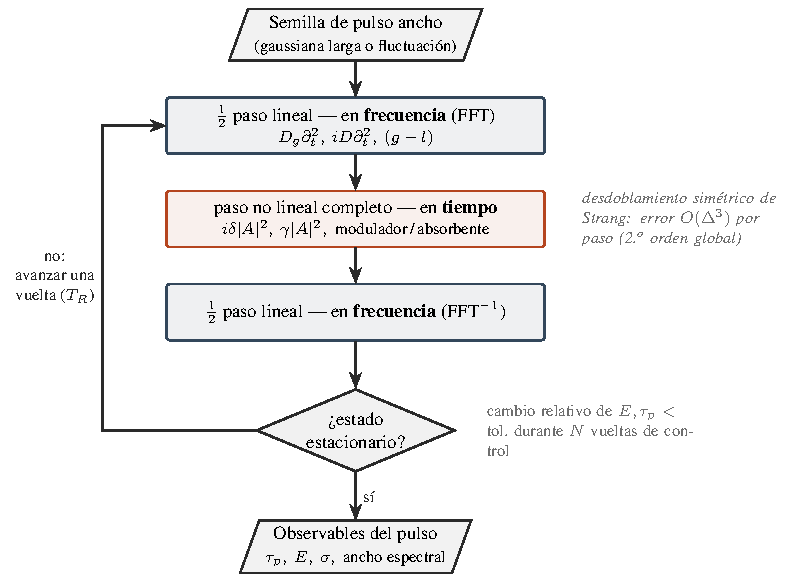
\includegraphics[width=0.82\textwidth]{chapters/images/ch4/fig_splitstep.pdf}
    \caption[Ciclo del integrador split-step]{Diagrama de flujo de una evaluación
    del simulador. A partir de una semilla de pulso ancho, cada vuelta de cavidad
    (paso de integración $=T_R$) se avanza con el desdoblamiento simétrico de
    Strang: medio paso lineal aplicado como multiplicador espectral (FFT), un paso
    no lineal completo aplicado punto a punto en el tiempo, y otro medio paso
    lineal. El ciclo se repite hasta que la envolvente alcanza el estado
    estacionario, del que se extraen los observables ($\tau_p$, $E$, $\sigma$,
    ancho espectral) que alimentan la función de mérito.}
    \label{fig:splitstep}
\end{figure}

La discretización sigue la práctica establecida para este tipo de simulación
\cite{Kaertner2020}: el \textbf{paso de integración en $T$ se toma igual al tiempo
de ida y vuelta $T_R$}, de modo que la acción discreta (por ronda) de la dispersión
y la no linealidad quede correctamente representada; la envolvente se muestrea sobre
una malla de $N$ puntos que cubre una ventana temporal mucho mayor que la duración
esperada del pulso, con una resolución temporal suficiente para resolver su perfil y
un ancho de banda espectral asociado suficiente para contener su espectro. La
condición inicial es una semilla de pulso ancho (una gaussiana larga o una
fluctuación de baja intensidad) que el propio proceso de bloqueo de modos acorta y
moldea hasta el pulso estacionario. Los valores concretos de $N$, de la ventana y
del número de vueltas simuladas se fijan en la Sección~\ref{sec:reproducibilidad} y
se justifican mediante las pruebas de convergencia de la
Sección~\ref{sec:sim_verificacion}.

\subsection{Criterio de estado estacionario y observables del pulso}
\label{sec:sim_estacionario}

Una evaluación del simulador termina cuando la envolvente alcanza el
\emph{estado estacionario}, esto es, cuando deja de cambiar de una vuelta a la
siguiente salvo el desfase global admitido por~\eqref{eq:haus_estacionario}. En la
práctica, la condición ideal $\partial A/\partial T=0$ se sustituye por un criterio
numérico de convergencia: las vueltas se agrupan en bloques de cien y se declara
alcanzado el régimen permanente cuando el cambio relativo de la energía media y de la
duración media entre bloques consecutivos queda por debajo de $10^{-6}$ durante cinco
bloques seguidos. Si eso no ocurre en $50\,000$ vueltas, el punto se declara no
convergido. Este estado se alcanza tras un
transitorio de miles de vueltas: en el caso de referencia de la
Sección~\ref{sec:sim_verificacion}, del orden de cuatro mil según Kärtner
\cite{Kaertner2020}, y de unas ocho mil cuatrocientas con el criterio de este trabajo,
que es más estricto. El número de vueltas hasta la convergencia no es un mero detalle
de implementación, sino una medida directa del \emph{costo} de una evaluación, que
la Sección~\ref{sec:metricas} incorpora como una de las métricas de comparación de
los algoritmos.

Del pulso estacionario se extrae el conjunto de \emph{observables} que resumen su
calidad y que alimentan la función de mérito (Sección~\ref{sec:funcion_merito}): la
duración $\tau_p$ a media altura, la energía $E$ y la intensidad de pico, el ancho
espectral y la proximidad de la forma al límite de transformada, y una medida de
\emph{estabilidad} $\sigma$, definida como el mayor de los coeficientes de variación de
la energía y de la duración dentro del último bloque. Esta medida complementa al
criterio de convergencia: una oscilación más rápida que un bloque deja constantes las
medias por bloque y pasaría inadvertida, pero no escapa a $\sigma$. La sensibilidad del
pulso a perturbaciones de los parámetros no entra en $\sigma$; se evalúa aparte, como
métrica de robustez (Sección~\ref{sec:metricas}). Estos
observables son la única información que el optimizador recibe de la física de la
cavidad: la función de mérito se construye enteramente a partir de ellos, sin acceso
a la forma interna de la ecuación maestra.

\subsection{Verificación del simulador}
\label{sec:sim_verificacion}

Antes de emplear el simulador como entorno de optimización se comprueba que
reproduce la física que pretende modelar, mediante tres pruebas complementarias.

La primera contrasta el pulso numérico con las \emph{soluciones analíticas} que la
ecuación maestra admite en sus límites tratables. En el régimen activo sin
dispersión ni no linealidad, el simulador recupera la gaussiana de
Kuizenga--Siegman y su ley de anchura $\tau\propto(D_g/M_s)^{1/4}$
(Sección~\ref{sec:kuizenga_siegman}); los valores de referencia publicados para
láseres representativos (del orden de $91$~ps para un Nd:YAG y $53$~ps para un
Nd:YLF con los parámetros habituales) fijan puntos de comparación cuantitativos
\cite{Keller2022}. En el régimen pasivo con absorbente rápido, la referencia es el
pulso de secante hiperbólica~\eqref{eq:pasivo_sech} con la
duración~\eqref{eq:tau_pasivo}. En el régimen de formación de solitón, la simulación
de referencia de Kärtner, que parte de una gaussiana larga y converge, tras unas
cuatro mil vueltas, a un pulso de $24$~ps en acuerdo exacto con la predicción
analítica, sirve de prueba de extremo a extremo del integrador
\cite{Kaertner2020}. El acuerdo entre el pulso estacionario numérico y estas
soluciones cerradas (del $0.01\%$ en el caso de Kuizenga--Siegman, con $91.42$~ps
frente a $91.41$~ps, y por debajo del $1\%$ en los otros dos) valida a la vez el modelo
y su implementación; los perfiles se presentan en la Sección~\ref{sec:res_validacion}.

La segunda prueba verifica que el simulador \emph{reproduce los regímenes de
operación conocidos} al recorrer el espacio de parámetros: la transición de onda
continua a bloqueo de modos de un solo pulso, y la aparición de operación
multipulso o de inestabilidades de \emph{Q\-/switching} en los límites del régimen
estable (Sección~\ref{sec:regimenes}). En el régimen pasivo, además, cada punto se evalúa
frente al margen de estabilidad respecto del \emph{Q\-/switching} que la
Sección~\ref{sec:restricciones} define como restricción del problema.

La tercera prueba es de \emph{consistencia numérica}: los observables del pulso
estacionario cambian menos del $0.05\%$ al reducir a la mitad o duplicar la malla
temporal $N$, al duplicar la ventana y al variar la tolerancia de convergencia en una
década, en ambos regímenes, de modo que las conclusiones no
dependan de la discretización elegida. Superadas las tres pruebas, el simulador
queda validado como entorno de evaluación y como generador de los datos con los que
la Sección~\ref{sec:formulacion_problema} plantea el problema de optimización.


% ============================================================
%  Seccion 4.2 -- Formulacion del problema de optimizacion (OE2)
% ============================================================

\section{Formulación del problema de optimización}
\label{sec:formulacion_problema}

El simulador de la Sección~\ref{sec:modelo_numerico} devuelve un pulso para cada configuración, pero todavía no un problema de optimización. Convertirlo en uno, el segundo objetivo específico, exige concretar sus tres ingredientes: fijar el vector de decisión y su dimensión en cada régimen, delimitar la región admisible con sus rangos físicos y su restricción de estabilidad, y adoptar una forma explícita para la función de mérito (Sección~\ref{sec:espacio_parametros}). Con ello queda definido, sin ambigüedad, el objetivo idéntico que maximizarán los tres algoritmos (Secciones~\ref{sec:ga}, \ref{sec:nnga} y~\ref{sec:pso}).

\subsection{Vector de decisión y dimensión efectiva por régimen}
\label{sec:decision_vector}

Las variables de decisión son los coeficientes de la ecuación maestra que resultan
ajustables en operación (Sección~\ref{sec:variables}), agrupados en el vector
$\mathbf{p}=(p_1,\dots,p_n)\in\mathcal{P}\subset\mathbb{R}^n$
\eqref{eq:vector_decision}. No todos los coeficientes de~\eqref{eq:sim_maestra} son
perillas: algunos quedan fijados por el diseño de la cavidad (las pérdidas lineales
$l$ por el acoplador de salida, y, en el régimen activo, la frecuencia de modulación
$\omega_m$, atada a la frecuencia de repetición de la cavidad), mientras que los
demás se varían durante la búsqueda. Distinguir unos de otros es lo que fija la
dimensión efectiva $n$ del problema.

En el \textbf{régimen activo}, las perillas son la ganancia de pequeña señal $g_0$
(gobernada por la potencia de bombeo; la ganancia saturada que entra en la ecuación
maestra resulta de $g=g_0/(1+E/E_{\mathrm{sat},L})$ \cite{Kaertner2020}), la dispersión neta por ronda $D$, el coeficiente de
automodulación de fase $\delta$ y la profundidad de modulación $M$:
%
\begin{equation}
    \mathbf{p}_{\text{act}} = (g_0,\, D,\, \delta,\, M) .
    \label{eq:decision_activo}
\end{equation}
%
En el \textbf{régimen pasivo}, el modulador externo se sustituye por el absorbente
saturable rápido, cuyos parámetros, la pérdida no saturada $q_0$ y el coeficiente de
automodulación de amplitud $\gamma$ (equivalentemente, la intensidad de saturación
$I_{\mathrm{sat},A}$), reemplazan a la profundidad de modulación:
%
\begin{equation}
    \mathbf{p}_{\text{pas}} = (g_0,\, D,\, \delta,\, q_0,\, \gamma) .
    \label{eq:decision_pasivo}
\end{equation}
%
La elección de modelado de la Sección~\ref{sec:sim_pasivo} (absorbente rápido ideal
y ganancia constante) es la que mantiene ambos vectores en una dimensión reducida y
comparable. Esta paridad es deliberada: como el estudio busca atribuir las
diferencias de desempeño al algoritmo y no a las particularidades del problema
(Sección~\ref{sec:aporte}), conviene que los dos regímenes planteen problemas de
dimensión similar. Aun así, el régimen activo conserva una estructura más
determinista y de menor dimensión efectiva (una perilla menos y sin la
realimentación intensidad\-/pérdida del absorbente), rasgo que la hipótesis de
trabajo (Sección~\ref{sec:hipotesis-alcance}) asocia a una convergencia más rápida y
que el estudio comparativo pondrá a prueba.

\subsection{Rangos físicos y restricciones}
\label{sec:restricciones}

La región admisible $\mathcal{P}$ queda delimitada, en primer lugar, por los
\emph{rangos físicos} de cada variable: cada perilla se acota entre los valores
mínimo y máximo accesibles en un montaje realista, lo que define una caja en
$\mathbb{R}^n$. Las escalas de esos rangos se toman de los valores característicos
documentados para los parámetros del absorbente (fluencia de saturación, tiempo de
recuperación, profundidad de modulación) y de los coeficientes de la ecuación
maestra \cite{Keller2022}; sus valores numéricos concretos se consignan en la
Sección~\ref{sec:reproducibilidad}.

A la restricción de caja se añade una \emph{restricción de estabilidad} propia del
régimen pasivo. Un absorbente saturable no solo sostiene el bloqueo de modos, sino
que, por debajo de cierta energía, empuja al láser a inestabilidades de
\emph{Q\-/switching} que impiden el tren de pulsos estable
(Sección~\ref{sec:regimenes}). % [REV-2026-11-17] criterio anti-QML reescrito: es el que implementa constraints.stability_margin
El criterio de Hönninger et al.\ \cite{Honninger1999}, tal como lo expone Keller
\cite{Keller2022}, establece que el bloqueo de modos es estable cuando, ante una
fluctuación de la energía, la saturación de la ganancia la frena más de lo que el
blanqueo del absorbente la amplifica. Para un absorbente lento ese criterio toma la
forma cerrada $E_p^{2}>E_{\mathrm{sat},L}E_{\mathrm{sat},A}\Delta R$. Como este trabajo
emplea un absorbente rápido (Sección~\ref{sec:sim_pasivo}), que no tiene los parámetros
$E_{\mathrm{sat},A}$ ni $\Delta R$, el criterio se evalúa directamente sobre el pulso
estacionario mediante el margen
%
\begin{equation}
    \mathcal{M} \;=\; s_g - s_q \;>\; 0,
    \qquad
    s_g = E\left|\frac{\partial g}{\partial E}\right|,
    \quad
    s_q = E\left|\frac{\partial q_p}{\partial E}\right|,
    \label{eq:restriccion_qml}
\end{equation}
%
donde $q_p(E)=E^{-1}\int q\,|A|^2\,dt$ es la pérdida del absorbente promediada sobre el
pulso. La derivada de la ganancia se obtiene de la ley de saturación,
$s_g=g\,x/(1+x)$ con $x=E/E_{\mathrm{sat},L}$; la del absorbente se calcula
numéricamente, escalando en $\pm5\%$ la energía del pulso final con su forma fija, y
solo cuenta cuando la pérdida disminuye con la energía, que es el caso
desestabilizador. En el régimen activo no hay absorbente, $s_q=0$, y el margen es
siempre positivo.

% [REV-2026-11-17] clasificador de régimen (constraints.classify), antes no descrito
La segunda restricción es operar en bloqueo de modos de un solo pulso. Para imponerla,
cada simulación se clasifica a partir de su estado final en uno de siete regímenes, en
este orden: divergido (campo no finito), extinto (energía menor que $10^{-18}$~J),
inestable ($\sigma>10^{-2}$), no convergido (sin estado estacionario tras el máximo de
vueltas), onda continua (fondo mediano por encima del $15\%$ del pico), multipulso (más
de una región por encima del $30\%$ del pico) y monopulso. Los umbrales se fijaron en
este trabajo. Solo el monopulso con margen~\eqref{eq:restriccion_qml} positivo es
admisible; la Sección~\ref{sec:funcion_merito_op} incorpora estas restricciones a la
función objetivo como penalización.

\subsection{La función de mérito}
\label{sec:funcion_merito_op}

La función de mérito $F(\mathbf{p})$ asigna a cada configuración un valor que mide la
calidad del pulso que produce, construido a partir de los observables del estado
estacionario que devuelve el simulador (Sección~\ref{sec:sim_estacionario}): la
duración $\tau_p$, la energía $E$ o intensidad de pico, el ancho espectral y la
proximidad al límite de transformada, y la estabilidad $\sigma$. El problema se
enuncia como la búsqueda del punto que maximiza el mérito dentro de la región
admisible,
$\mathbf{p}^\star=\arg\max_{\mathbf{p}\in\mathcal{P}} F(\mathbf{p})$
\eqref{eq:problema_optimizacion}.

De los dos enfoques que admite su construcción (Sección~\ref{sec:funcion_merito}),
este trabajo adopta la \textbf{función de mérito escalar}: los objetivos se combinan
en un único número mediante una suma ponderada que premia el pulso más corto,
energético y estable, y penaliza las configuraciones que caen fuera del régimen de
bloqueo de modos de un solo pulso,
%
\begin{equation}
    F(\mathbf{p}) = w_1\,\frac{1}{\tau_p}
    + w_2\,E - w_3\,\sigma - \Pi(\mathbf{p}),
    \label{eq:merito_op}
\end{equation}
%
donde $\sigma$ cuantifica la inestabilidad del tren de pulsos y $\Pi(\mathbf{p})$ es
el término de penalización que se aplica cuando se violan las restricciones de
la Sección~\ref{sec:restricciones}, en particular, cuando no se satisface la
condición de estabilidad~\eqref{eq:restriccion_qml} o el punto cae en un régimen
indeseado. Es la forma escalar descrita en la
Sección~\ref{sec:funcion_merito}, que aquí se fija como objetivo de trabajo.
% [REV-2026-11-23] antes remitía a eq:merito_escalar, eliminada del cap. 3

% [REV-2026-11-17] implementación real del mérito (problem/merit.py)
En la implementación, cada término se adimensionaliza con una escala de referencia para
que los pesos sean de orden uno y comparables,
%
\begin{equation}
    F(\mathbf{p}) = w_\tau\,\frac{\tau_{\mathrm{ref}}}{\tau_p}
    + w_E\,\frac{E}{E_{\mathrm{ref}}} - w_\sigma\,\frac{\sigma}{\sigma_{\mathrm{ref}}}
    - \Pi(\mathbf{p}),
    \label{eq:merito_adim}
\end{equation}
%
con $\tau_{\mathrm{ref}}=10$~ps, $E_{\mathrm{ref}}=40$~nJ y $\sigma_{\mathrm{ref}}=10^{-3}$,
lo que equivale a~\eqref{eq:merito_op} con $w_1=w_\tau\tau_{\mathrm{ref}}$,
$w_2=w_E/E_{\mathrm{ref}}$ y $w_3=w_\sigma/\sigma_{\mathrm{ref}}$. Normalizar los objetivos
antes de sumarlos es la práctica recomendada para la suma ponderada
\cite{MarlerArora2010}. Los pesos $(w_\tau,w_E,w_\sigma)=(1,\,0.5,\,0.5)$ expresan una
preferencia y no un óptimo: la duración es el objetivo principal, y la energía y la
estabilidad, secundarios. La escala $E_{\mathrm{ref}}$ se fijó tras una corrida piloto
(Sección~\ref{sec:calibracion_piloto}).

La penalización no es plana. Un punto infactible recibe $F=-(\Pi_0+\Pi_1 v)$, con
$\Pi_0=\Pi_1=10$ y $v\in[0,2]$ una medida de la gravedad de la violación que crece con
la distancia al régimen admisible: $v\le0.5$ para un monopulso con margen negativo,
$v=0.5$ para un punto no convergido, $v\in(0.5,1]$ para uno inestable según su
$\sigma$, $v=0.75$ para el multipulso, $v=1$ para la onda continua y $v=2$ para un campo
divergido o extinto. Como todo punto factible tiene $F>0$ y todo punto infactible
$F\le-10$, el esquema reproduce las reglas de factibilidad de Deb \cite{Deb2000}: un
punto factible siempre supera a uno infactible, y entre dos infactibles gana el que
viola menos. La gradación orienta la búsqueda cuando buena parte de la población es
infactible. No se comparó con una penalización plana. La Figura~\ref{fig:merito} esquematiza su construcción a partir de los
observables.

\begin{figure}[t]
    \centering
    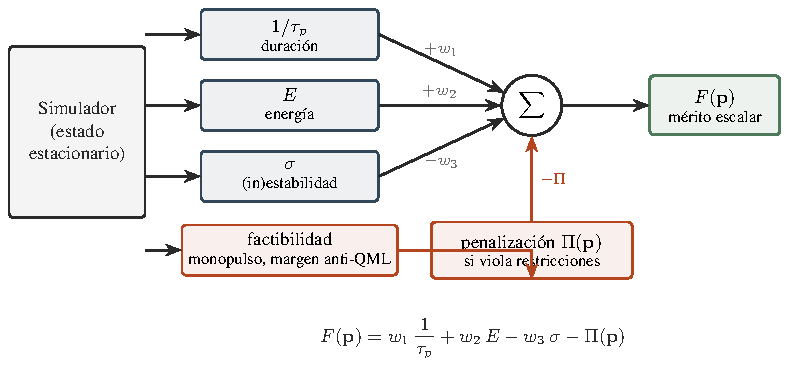
\includegraphics[width=0.92\textwidth]{chapters/images/ch4/fig_merito.pdf}
    \caption[Construcción de la función de mérito escalar]{Construcción de la
    función de mérito escalar~\eqref{eq:merito_op}. Los observables del pulso
    estacionario que devuelve el simulador (la duración $\tau_p$, la energía $E$ y
    la estabilidad $\sigma$) se combinan en una suma ponderada que premia el pulso
    más corto, energético y estable. Una comprobación de factibilidad (régimen de
    monopulso, margen anti-\emph{Q\-/switching}) activa la penalización
    $\Pi(\mathbf{p})$, que sitúa a todo punto infactible por debajo de cualquier
    punto factible. El resultado
    es el escalar $F(\mathbf{p})$ que los tres algoritmos maximizan.}
    \label{fig:merito}
\end{figure}

La elección del enfoque escalar frente al multiobjetivo obedece al diseño del
estudio. Su núcleo es una comparación controlada en la que el láser, el espacio de
parámetros y la función de mérito permanecen fijos y solo varía el algoritmo
(Sección~\ref{sec:aporte}); una única función objetivo escalar es lo que permite
enfrentar a los tres métodos sobre exactamente la misma meta y comparar su
desempeño con las mismas métricas (Sección~\ref{sec:metricas}), sin la
ambigüedad que introduciría contrastar frentes de Pareto de distinta forma. El
enfoque multiobjetivo, que expondría explícitamente los compromisos entre duración,
energía y estabilidad, queda como una extensión natural del protocolo, fuera del
estudio comparativo central. Los pesos $w_i$ y la forma precisa de la penalización
$\Pi$ se fijan en la Sección~\ref{sec:reproducibilidad}, y se mantienen idénticos
para los tres algoritmos.

\subsection{El problema como caja negra sin gradiente}
\label{sec:caja_negra}

Con las variables~\eqref{eq:decision_activo}--\eqref{eq:decision_pasivo}, la región
admisible $\mathcal{P}$ y el objetivo~\eqref{eq:merito_op}, el problema de
optimización queda completamente planteado. Su naturaleza determina qué clase de
método puede resolverlo. La función $F(\mathbf{p})$ no se conoce en forma cerrada:
cada evaluación exige integrar la ecuación maestra hasta el estado estacionario
(Sección~\ref{sec:sim_integracion}), un cómputo de miles de vueltas que no
proporciona derivadas de la salida respecto de las variables. El espacio, además, es
fuertemente acoplado, no convexo y multiestable, la lectura de la ecuación maestra
pasiva como una ecuación de Ginzburg--Landau compleja, con su variedad de
atractores, es el origen físico de esa multiplicidad de óptimos
(Secciones~\ref{sec:sim_pasivo} y~\ref{sec:estructura_espacio})
\cite{Kaertner2020}.

Estos rasgos (evaluación costosa de caja negra, ausencia de gradiente y paisaje
multimodal) descartan el ajuste manual y los métodos basados en gradiente, y
justifican el recurso a la optimización \emph{global} y \emph{libre de derivadas}
\cite{Genty2021}. Las tres estrategias que compara esta tesis, el algoritmo genético
(Sección~\ref{sec:ga}), la red neuronal acoplada al algoritmo genético
(Sección~\ref{sec:nnga}) y la optimización por enjambre de partículas
(Sección~\ref{sec:pso}), pertenecen todas a esa familia y comparten el paradigma de
explorar el espacio a partir únicamente de evaluaciones de $F$, difiriendo de forma
controlada en la mecánica de la búsqueda. Las secciones siguientes desarrollan cada
una de ellas.


% ============================================================
%  Seccion 4.3 -- Algoritmo genetico (OE3)
% ============================================================

\section{Algoritmo genético}
\label{sec:ga_impl}

El algoritmo genético (GA) es la línea base del estudio, la referencia frente a la cual se contrastan las otras dos estrategias; se elige por su madurez y por ser el método más asentado en la autooptimización de láseres ultrarrápidos \cite{Andral2015,Woodward2016}. Sobre sus operadores y su ciclo generacional (Sección~\ref{sec:ga}), esta sección fija las decisiones de implementación con que se aplica al problema de la Sección~\ref{sec:formulacion_problema}: cómo se representa e inicializa la población, qué variantes de los operadores se emplean y cómo se tratan las restricciones, y qué hiperparámetros y criterios de parada gobiernan la búsqueda.

\subsection{Representación e inicialización}
\label{sec:ga_representacion}

Cada individuo de la población es un vector de decisión $\mathbf{p}$
(Sección~\ref{sec:decision_vector}), codificado directamente como una cadena de
números reales cuyos genes son los parámetros ajustables de la cavidad. Se adopta,
por tanto, una \emph{codificación real} en lugar de la binaria clásica: como las
variables de la ecuación maestra son continuas, la codificación real evita la
discretización artificial de los genes, respeta la topología del espacio y permite
operadores de cruce y mutación que actúan sobre los valores físicos de los
parámetros (Sección~\ref{sec:ga_metafora}). El mismo esquema sirve a los dos
regímenes: la única diferencia es la longitud del cromosoma, dada por la dimensión
del vector correspondiente, cuatro genes en el activo \eqref{eq:decision_activo},
cinco en el pasivo \eqref{eq:decision_pasivo}.

La población inicial se genera por muestreo \emph{aleatorio uniforme} dentro de la
región admisible $\mathcal{P}$: cada gen se sortea de manera independiente entre los
límites físicos de su parámetro (Sección~\ref{sec:restricciones}), de modo que la
primera generación cubre la caja de búsqueda sin sesgo hacia ninguna región. La
aptitud de cada individuo es el valor de la función de mérito $F(\mathbf{p})$
\eqref{eq:merito_op}, que se obtiene integrando la cavidad hasta el estado
estacionario y evaluando los observables del pulso resultante
(Sección~\ref{sec:sim_estacionario}); las configuraciones que violan las
restricciones, en particular la de estabilidad frente al \emph{Q\-/switching}
\eqref{eq:restriccion_qml}, reciben la penalización $\Pi(\mathbf{p})$ que las relega
en la selección. Esta incorporación del conocimiento fenomenológico a la aptitud
(penalizar los atractores degenerados y premiar el pulso único) es la que la
literatura identifica como determinante para la convergencia global del GA en este
tipo de problema \cite{Woodward2016}.

\subsection{Operadores genéticos y ciclo}
\label{sec:ga_operadores_impl}

La evolución de una generación a la siguiente se articula con las tres operaciones
descritas en la Sección~\ref{sec:ga_operadores}, para las que se fijan las siguientes
variantes concretas.

\begin{itemize}
    \item \textbf{Selección por torneo.} Los progenitores se eligen enfrentando
    subconjuntos pequeños de individuos tomados al azar y quedándose con el de mayor
    aptitud de cada torneo. Se prefiere al muestreo proporcional
    \eqref{eq:ga_seleccion} por su robustez frente a diferencias extremas de mérito, frecuentes en un paisaje con penalizaciones abruptas, y porque su presión
    selectiva se ajusta de forma sencilla con el tamaño del torneo.

    \item \textbf{Cruce aritmético.} Dos progenitores $\mathbf{p}_a$ y
    $\mathbf{p}_b$ engendran descendencia por combinación convexa de sus genes,
    $\mathbf{p}_{\text{hijo}}=\alpha\,\mathbf{p}_a+(1-\alpha)\,\mathbf{p}_b$ con
    $\alpha\in[0,1]$, lo que mantiene a los hijos dentro de la caja y explora el
    interior de la región que ocupan los buenos individuos. Una variante de mezcla
    (\emph{blend}), que extiende ligeramente el intervalo entre progenitores, se
    contempla para reforzar la exploración cuando la población empieza a concentrarse.

    \item \textbf{Mutación gaussiana.} Con baja probabilidad, cada gen se perturba
    sumándole un incremento gaussiano de media nula y desviación proporcional al
    rango del parámetro. Introduce diversidad nueva, evita la convergencia prematura
    a un óptimo local y sostiene la exploración del espacio multiestable.
\end{itemize}

Tras el cruce y la mutación, los genes que se salgan de sus límites se \emph{recortan}
(o se vuelven a muestrear) al borde de la caja, garantizando que todo individuo
permanezca en $\mathcal{P}$. Se aplica además \emph{elitismo}: los mejores individuos
pasan sin alteración a la generación siguiente, de modo que la mejor solución hallada
nunca se pierde. El ciclo (evaluación de la aptitud, selección, cruce, mutación y
reemplazo con elitismo) se repite generación tras generación
(Sección~\ref{sec:ga_ciclo}), desplazando la población hacia zonas de mérito
creciente mientras la mutación preserva la diversidad necesaria para no estancarse
(Figura~\ref{fig:ga-flujo}).

\begin{figure}[t]
    \centering
    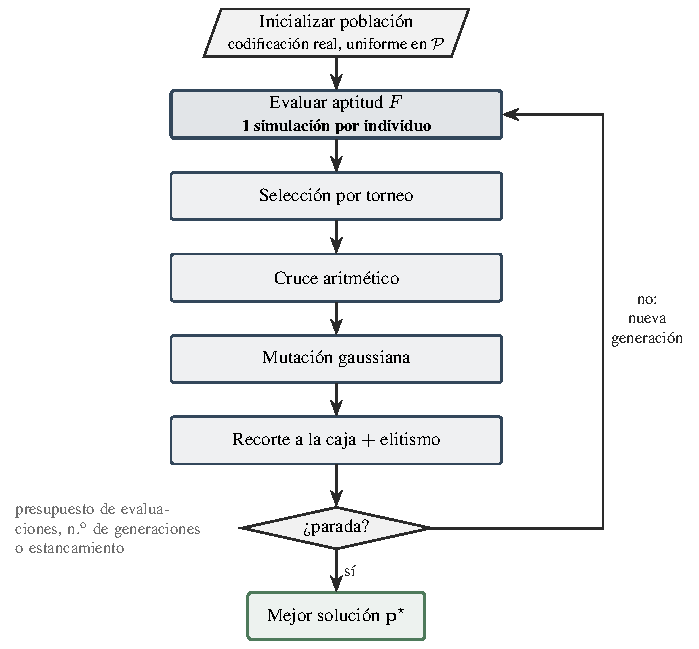
\includegraphics[width=0.62\textwidth]{chapters/images/ch4/fig_ga_flujo.pdf}
    \caption[Ciclo del algoritmo genético]{Ciclo generacional del algoritmo
    genético. Cada individuo es un vector de decisión con codificación real; su
    aptitud requiere una simulación completa de la cavidad (la operación
    dominante del costo). La generación evoluciona por selección de torneo, cruce
    aritmético y mutación gaussiana, con recorte a la caja y elitismo, hasta
    satisfacer un criterio de parada (agotar el presupuesto de evaluaciones,
    alcanzar un número de generaciones o estancarse).}
    \label{fig:ga-flujo}
\end{figure}

\subsection{Hiperparámetros y criterios de parada}
\label{sec:ga_hiperparametros}

El comportamiento del GA queda fijado por un conjunto de hiperparámetros: el tamaño
de la población, las probabilidades de cruce y de mutación (y la amplitud del paso de
mutación), el tamaño del torneo de selección y el número de individuos preservados
por elitismo. Su elección gobierna el equilibrio entre exploración y explotación y
se documenta, junto con sus valores concretos, en la Sección~\ref{sec:reproducibilidad},
donde se fija de manera idéntica para los dos regímenes a fin de no introducir
diferencias ajenas al algoritmo. 
% [REV-2026-11-17] valores y su justificación
Los valores son los habituales para codificación real en pocas dimensiones: población
de $20$, torneo de $3$, probabilidad de cruce de $0.9$, mutación por gen de $0.15$
(cercana a $1/n$ para $n=4$ o $5$) con desviación del $10\%$ del rango, y dos individuos
de élite. No se ajustaron por régimen ni por método: ajustarlos favorecería al método
mejor sintonizado, de modo que mantenerlos fijos es parte del diseño controlado, aunque
también un límite del estudio.

La búsqueda se detiene por cualquiera de tres criterios: alcanzar un número máximo de
generaciones, agotar un \emph{presupuesto de evaluaciones} del simulador prefijado, o
estancarse, cuando la mejora de la mejor aptitud entre generaciones sucesivas cae por
debajo de un umbral durante un número dado de generaciones. El presupuesto de
evaluaciones se adopta como criterio principal porque es la magnitud que hace
comparables a los tres métodos: como cada evaluación de la aptitud exige una
simulación completa de la cavidad, la operación dominante del proceso
(Sección~\ref{sec:caja_negra}), el número total de llamadas al simulador, producto
del tamaño de la población por el número de generaciones, es la medida natural del
costo y una de las métricas de comparación (Sección~\ref{sec:metricas}).

Este mismo costo es el que define el papel del GA en el estudio. Como línea base,
proporciona la referencia de calidad y de presupuesto contra la que se miden las
otras dos estrategias: la red neuronal acoplada (Sección~\ref{sec:nnga}) buscará
alcanzar una calidad comparable con menos llamadas al simulador, sustituyendo la
mayoría de las evaluaciones por un modelo aprendido más barato, y la optimización por
enjambre (Sección~\ref{sec:pso}) contrastará una mecánica de búsqueda distinta sobre
el mismo presupuesto.


% ============================================================
%  Seccion 4.4 -- Red neuronal sustituta acoplada al GA (OE4)
% ============================================================

\section{Red neuronal como sustituto acoplada al algoritmo genético}
\label{sec:nnga_impl}

El algoritmo genético busca con solvencia, pero cada una de sus miles de evaluaciones exige una simulación completa de la cavidad. La segunda estrategia ataca ese costo: una red neuronal que actúe como sustituto del simulador, acoplada al algoritmo genético para reemplazar la mayoría de esas simulaciones por predicciones baratas (cuarto objetivo específico). Esta sección fija las decisiones de implementación de ese esquema: la arquitectura del perceptrón multicapa (Sección~\ref{sec:mlp}), su entrenamiento supervisado (Sección~\ref{sec:entrenamiento}) y el bucle de acoplamiento con verificación (Sección~\ref{sec:surrogate_acoplamiento}).

\subsection{Arquitectura del sustituto y datos de entrenamiento}
\label{sec:nnga_arquitectura}

El modelo sustituto es un perceptrón multicapa que toma como entrada el vector de
decisión $\mathbf{p}$ (Sección~\ref{sec:decision_vector}) y devuelve una predicción
de los observables del pulso estacionario. Se adopta una decisión de diseño
deliberada: en lugar de predecir directamente el valor escalar de la función de
mérito, la red predice los \emph{observables físicos} (la duración $\tau_p$, la
energía $E$ o intensidad de pico y la medida de estabilidad $\sigma$) a partir de los
cuales se calcula después $F(\mathbf{p})$ con la expresión~\eqref{eq:merito_op}. Este
esquema, el mismo que la literatura consolida para el patrón NN+GA
\cite{Han2024}, tiene dos ventajas sobre la predicción directa de $F$: desacopla el
sustituto de los pesos de la función de mérito, de modo que estos pueden ajustarse
sin reentrenar la red, y permite aplicar las restricciones y la penalización
$\Pi(\mathbf{p})$ (Sección~\ref{sec:restricciones}) sobre observables interpretables.
% [REV-2026-11-17] arquitectura real (optimizers/nnga/surrogate.py)
La red tiene un tronco común de dos capas ocultas de $64$ neuronas con activación ReLU
y dos salidas. Una cabeza de regresión predice $(\tau_p, E, \sigma)$ y se entrena solo
con las muestras factibles; una cabeza de clasificación estima la probabilidad de que el
punto sea factible y se entrena con todas. La segunda cabeza es necesaria porque la
factibilidad (monopulso y margen positivo) no se deduce de los observables predichos.
Si la probabilidad estimada es menor que $0.5$, el punto recibe la penalización base;
si no, su mérito se calcula con~\eqref{eq:merito_adim} sobre los observables predichos.
Como $\tau_p$ y $\sigma$ abarcan varias décadas, se predicen en escala logarítmica.
La Figura~\ref{fig:red-arquitectura} ilustra este esquema.

\begin{figure}[t]
    \centering
    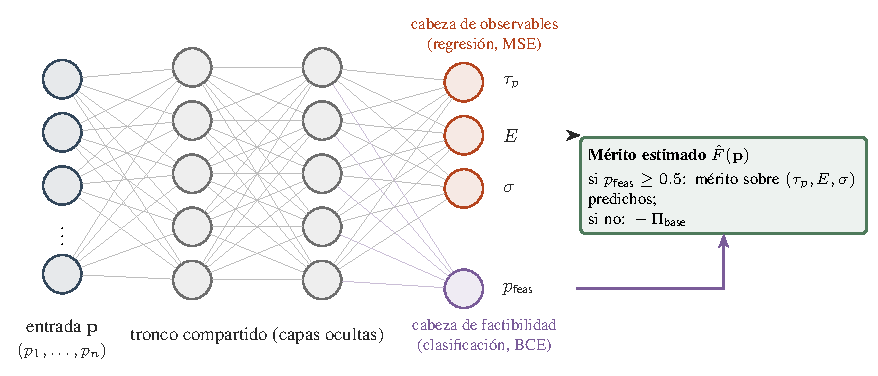
\includegraphics[width=0.86\textwidth]{chapters/images/ch4/fig_red_arquitectura.pdf}
    \caption[Arquitectura del sustituto neuronal]{Arquitectura del sustituto: un
    perceptrón multicapa con un \emph{tronco compartido} de capas ocultas y
    \emph{dos cabezas}. La cabeza de observables (regresión, entrenada por error
    cuadrático medio sobre las muestras factibles) predice
    $\hat{\mathbf{y}}=(\tau_p, E, \sigma)$ en lugar del valor de mérito; la cabeza
    de factibilidad (clasificación, entrenada por entropía cruzada sobre todas las
    muestras) estima la probabilidad $p_{\text{feas}}$ de que la configuración caiga
    en el régimen de monopulso estable, una decisión que no es derivable de los
    observables $(\tau_p,E,\sigma)$ predichos,. El mérito estimado
    $\hat{F}(\mathbf{p})$ evalúa la rama factible del mérito~\eqref{eq:merito_op}
    sobre los observables predichos cuando $p_{\text{feas}}\ge 0.5$, y devuelve la
    penalización base $-\Pi_{\text{base}}$ en caso contrario. Predecir observables
    interpretables, y no $F$ directamente, desacopla el sustituto de los pesos de
    la función de mérito y permite imponer las restricciones sobre magnitudes
    físicas.}
    \label{fig:red-arquitectura}
\end{figure}

El conjunto de datos de entrenamiento se genera ejecutando el simulador sobre un
muestreo del espacio de parámetros: se sortean configuraciones $\mathbf{p}^{(k)}$
dentro de la región admisible $\mathcal{P}$ (mediante un muestreo que cubra el
espacio de forma homogénea, como el hipercubo latino, más eficiente que el sorteo
puramente aleatorio) y, para cada una, se integra la cavidad hasta el estado
estacionario y se registran sus observables, formando los pares
$\{(\mathbf{p}^{(k)}, \mathbf{y}^{(k)})\}$ con $\mathbf{y}$ el vector de observables.
Las entradas y las salidas se \emph{normalizan} a rangos comparables para facilitar
el entrenamiento. Este muestreo inicial consume una parte del presupuesto de
simulaciones, la inversión que el método debe amortizar, y se contabiliza
explícitamente en el costo total (Sección~\ref{sec:nnga_acoplamiento}). Se toman $40$
puntos, del orden de los diez por dimensión que se recomiendan para el diseño inicial
de un experimento computacional \cite{Loeppky2009}. El conjunto se divide en subconjuntos de
entrenamiento y validación para vigilar la generalización.

\subsection{Entrenamiento y validación}
\label{sec:nnga_entrenamiento}

Los pesos y sesgos de la red, $\boldsymbol{\theta}$, se ajustan por aprendizaje
supervisado (Sección~\ref{sec:entrenamiento}), minimizando, en la cabeza de regresión, el error cuadrático medio
entre las predicciones y los observables simulados (la cabeza de factibilidad minimiza
la entropía cruzada binaria),
%
\begin{equation}
    \mathcal{L}(\boldsymbol{\theta})
    = \frac{1}{K}\sum_{k=1}^{K}
    \bigl\lVert\, \hat{\mathbf{y}}_{\boldsymbol{\theta}}(\mathbf{p}^{(k)})
    - \mathbf{y}^{(k)} \,\bigr\rVert^2,
    \label{eq:nnga_perdida}
\end{equation}
%
una generalización de la pérdida~\eqref{eq:perdida_mse} al vector de observables. La
minimización se realiza por descenso de gradiente estocástico con
retropropagación, empleando el optimizador adaptativo Adam; el
optimizador concreto, la tasa de aprendizaje y el tamaño de lote se fijan en la
Sección~\ref{sec:reproducibilidad}. Para evitar el sobreajuste se vigila el error
sobre el subconjunto de validación y se detiene el entrenamiento cuando ese error
deja de mejorar (\emph{parada temprana}), complementado con las técnicas de
regularización habituales. La calidad del sustituto se juzga por su capacidad de
\emph{generalización}, el error de predicción sobre puntos no vistos, pues es esa
precisión, y no el ajuste sobre los datos de entrenamiento, la que determina si la
red puede reemplazar con fiabilidad al simulador dentro del ciclo de búsqueda.

\subsection{Esquema de acoplamiento NN+GA}
\label{sec:nnga_acoplamiento}

Una vez entrenado, el sustituto se integra en el mismo algoritmo genético de la
Sección~\ref{sec:ga_impl} (con idénticos operadores e hiperparámetros) reemplazando,
en la evaluación de la aptitud de cada individuo, la llamada al simulador por una
consulta a la red seguida del cálculo de $F$ sobre los observables predichos. Que la
maquinaria de búsqueda sea exactamente la del GA puro es lo que hace limpia la
comparación: entre las dos estrategias solo cambia la fuente de la aptitud, de modo
que cualquier diferencia de desempeño se atribuye al uso del sustituto y no a otra
variación del optimizador (Sección~\ref{sec:aporte}).

El acoplamiento no sustituye \emph{todas} las simulaciones, porque hacerlo expondría
la búsqueda a un riesgo conocido: si la red se equivoca en regiones poco
representadas, el algoritmo genético puede converger hacia soluciones que parecen
óptimas para el sustituto pero mediocres para el simulador real, «explotando» los
errores del modelo (Sección~\ref{sec:surrogate_acoplamiento}). Para contenerlo, el
esquema intercala una \emph{verificación selectiva}: de forma periódica, las mejores
soluciones que el GA propone sobre el sustituto se reevalúan con el simulador
auténtico; los nuevos pares $(\mathbf{p}, \mathbf{y})$ así obtenidos se incorporan al
conjunto de entrenamiento y la red se reajusta. Este bucle (búsqueda barata sobre el
sustituto, verificación con el simulador, reentrenamiento) concentra el escaso
presupuesto de simulaciones en las regiones de mayor mérito, que son las que de
verdad importan, y va mejorando el sustituto justo donde la búsqueda se detiene. La
Figura~\ref{fig:nnga-esquema} resume el esquema y su contabilidad de costo.

\begin{figure}[t]
    \centering
    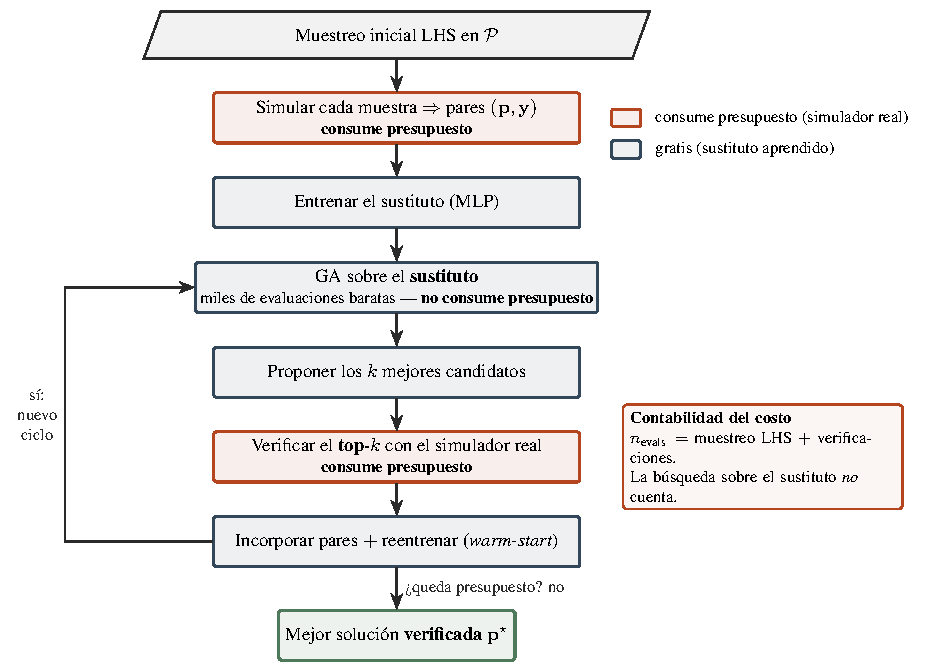
\includegraphics[width=0.92\textwidth]{chapters/images/ch4/fig_nnga_esquema.pdf}
    \caption[Esquema de acoplamiento NN+GA]{Esquema de acoplamiento NN+GA. Un
    muestreo inicial por hipercubo latino se simula para entrenar el sustituto;
    después, el mismo algoritmo genético de la Sección~\ref{sec:ga_impl} busca
    sobre el sustituto (miles de evaluaciones baratas que \emph{no} consumen
    presupuesto) y propone los $k$ mejores candidatos, que se \emph{verifican} con
    el simulador real; los nuevos pares reentrenan la red (\emph{warm-start}) y el
    ciclo se repite. Solo las llamadas al simulador (en color) cuentan para el
    costo: $n_{\text{evals}}=$ muestreo inicial $+$ verificaciones. El resultado
    es siempre la mejor solución \emph{verificada}.}
    \label{fig:nnga-esquema}
\end{figure}

La contabilidad del costo es, por tanto, la clave de la estrategia. El número total
de llamadas al simulador, la métrica que compara los métodos
(Sección~\ref{sec:metricas}), es la suma de las que consume el muestreo inicial de
entrenamiento y las de las verificaciones periódicas. En este trabajo son $40$ puntos
iniciales más seis ciclos de cinco verificaciones: setenta evaluaciones reales, frente a
las cuatrocientas del presupuesto de los otros dos métodos. Si ese ahorro se materializa sin sacrificar la calidad del pulso,
y bajo qué condiciones, es precisamente una de las preguntas empíricas que el
estudio comparativo busca responder (Sección~\ref{sec:hipotesis-alcance}). La
tercera estrategia aborda el mismo problema desde una filosofía de búsqueda distinta
(la inteligencia de enjambre) y es el objeto de la sección siguiente.


% ============================================================
%  Seccion 4.5 -- Optimizacion por enjambre de particulas (OE5)
% ============================================================

\section{Optimización por enjambre de partículas}
\label{sec:pso_impl}

La tercera estrategia, la optimización por enjambre de partículas (PSO), aborda el mismo problema con una mecánica de búsqueda distinta: un enjambre de partículas que se mueven guiadas por su memoria personal y colectiva, sin operadores de recombinación (Sección~\ref{sec:pso}). Se elige por su uso bien documentado en la optimización de láseres de modos bloqueados, donde gestiona con robustez funciones de aptitud discontinuas y fuertemente no lineales \cite{Kokhanovskiy2021,Nsoungui2026}. Esta sección concreta las decisiones de implementación con que se aplica al problema de la Sección~\ref{sec:formulacion_problema}.

\subsection{Partículas, dinámica y topología}
\label{sec:pso_dinamica_impl}

Cada partícula del enjambre representa una solución candidata mediante su posición
$\mathbf{x}_i$ en el espacio de parámetros, el análogo del vector de decisión
$\mathbf{p}$ (Sección~\ref{sec:decision_vector}), y se desplaza por él con una
velocidad $\mathbf{v}_i$ (Sección~\ref{sec:pso_particulas}). El enjambre se
inicializa sorteando las posiciones de forma \emph{aleatoria uniforme} dentro de la
región admisible $\mathcal{P}$, igual que la población inicial del algoritmo genético
(Sección~\ref{sec:ga_representacion}), para no introducir sesgos de partida ajenos al
método, y las velocidades con valores pequeños. La aptitud que gobierna la búsqueda
es la misma función de mérito $F(\mathbf{p})$ \eqref{eq:merito_op} evaluada por el
simulador, de modo que cada partícula recuerda su mejor posición personal
$\mathbf{p}_i^{\text{best}}$ y el enjambre comparte la mejor posición global
$\mathbf{g}^{\text{best}}$.

En cada iteración, la velocidad y la posición de cada partícula se actualizan según
la regla de la Sección~\ref{sec:pso_dinamica}, que combina inercia, atracción hacia
la mejor experiencia propia y atracción hacia la mejor colectiva
\eqref{eq:pso_velocidad}--\eqref{eq:pso_posicion}. Sobre esa regla se fijan tres
decisiones de implementación. Primero, el \emph{peso de inercia} $\omega$ se reduce
de forma progresiva a lo largo de las iteraciones, de un valor alto que privilegia la
exploración global al comienzo a uno bajo que favorece la convergencia local al
final; es el principal regulador del compromiso entre exploración y explotación
(Sección~\ref{sec:pso_dinamica}). Segundo, para impedir que las partículas adquieran
velocidades excesivas que las hagan rebasar las buenas regiones, la velocidad se
\emph{acota} a un máximo por dimensión (\emph{velocity clamping}). Tercero, cuando
una partícula abandona la caja de búsqueda, su posición se \emph{recorta} al borde de
$\mathcal{P}$ y su velocidad en esa dimensión se anula o invierte, con lo que el
enjambre respeta las mismas restricciones físicas que los demás métodos
(Sección~\ref{sec:restricciones}). En cuanto a la \emph{topología} de comunicación,
se adopta la global (todas las partículas consultan un único
$\mathbf{g}^{\text{best}}$) por su convergencia rápida, contemplando una topología
local en vecindario como variante para preservar la diversidad si se observa
estancamiento prematuro. La
Figura~\ref{fig:pso-flujo} resume el ciclo del enjambre.

\begin{figure}[t]
    \centering
    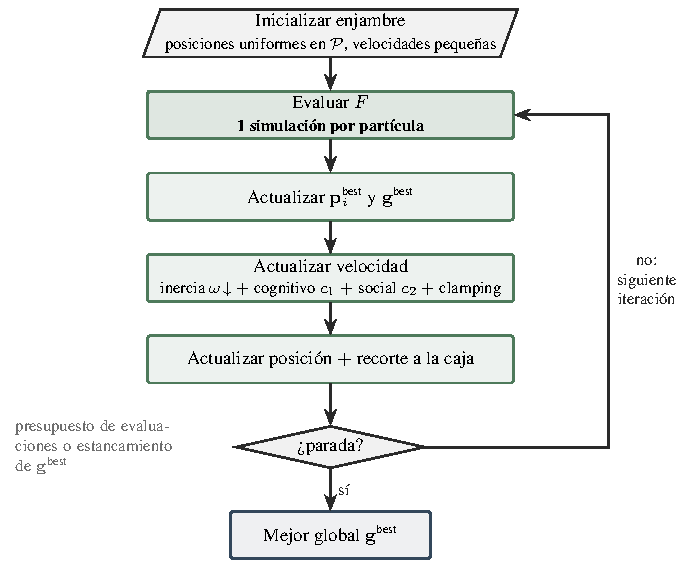
\includegraphics[width=0.66\textwidth]{chapters/images/ch4/fig_pso_flujo.pdf}
    \caption[Ciclo de la optimización por enjambre]{Ciclo de la optimización por
    enjambre de partículas. Cada partícula evalúa la misma función de mérito con el
    simulador y actualiza su mejor posición personal $\mathbf{p}_i^{\text{best}}$ y
    la mejor global $\mathbf{g}^{\text{best}}$; su velocidad combina inercia
    decreciente, atracción cognitiva y social, con acotación (\emph{clamping}), y
    su posición se recorta a la caja. El ciclo se repite hasta agotar el
    presupuesto de evaluaciones o estancarse. Frente al algoritmo genético,
    prescinde de operadores de recombinación y tiene menos hiperparámetros que
    ajustar.}
    \label{fig:pso-flujo}
\end{figure}

\subsection{Hiperparámetros y criterios de parada}
\label{sec:pso_hiperparametros}

El comportamiento del PSO queda fijado por un conjunto de hiperparámetros más
reducido que el del algoritmo genético: el tamaño del enjambre, el esquema de
variación del peso de inercia $\omega$, los coeficientes de aceleración cognitivo
$c_1$ y social $c_2$, la cota de velocidad máxima y la topología del enjambre. Sus
valores concretos se documentan en la Sección~\ref{sec:reproducibilidad}.
% [REV-2026-11-17] valores y su respaldo
El enjambre tiene $20$ partículas y topología global. El peso de inercia decrece
linealmente de $0.9$ a $0.4$, el esquema de Shi y Eberhart \cite{ShiEberhart1998};
$c_1=c_2=1.5$, próximos al valor $1.49445$ que se deriva del factor de constricción
\cite{ClercKennedy2002,EberhartShi2000}; la velocidad se limita al $20\%$ del rango y,
si una partícula sale de la caja, su posición se recorta al borde y su velocidad se
anula. Como en el GA, estos valores no se ajustaron. Esta
economía de parámetros (una implementación con menos elementos que ajustar que la del
GA) es, junto con su convergencia inicial típicamente rápida, uno de los rasgos que
distinguen al método (Sección~\ref{sec:pso_topologia}).

La búsqueda se detiene, como en las demás metaheurísticas, al agotar el
\emph{presupuesto de evaluaciones} del simulador o cuando el mejor global
$\mathbf{g}^{\text{best}}$ deja de mejorar durante un número dado de iteraciones. Que
el criterio principal sea el presupuesto de evaluaciones no es casual: es la
condición que hace \emph{comparable} al PSO con las otras dos estrategias. El estudio
enfrenta a los tres métodos sobre el mismo simulador, el mismo espacio $\mathcal{P}$,
la misma función de mérito y el mismo presupuesto de llamadas al simulador, variando
únicamente el algoritmo (Sección~\ref{sec:aporte}); solo así las diferencias que se
observen en las métricas de calidad, costo y robustez (Sección~\ref{sec:metricas})
podrán atribuirse a la mecánica de búsqueda (la recombinación evolutiva del GA, el
sustituto aprendido del NN+GA o el movimiento social del enjambre) y no a las
particularidades del problema. Con las tres estrategias ya especificadas, la sección
siguiente define ese protocolo comparativo y las métricas con que se juzga su
desempeño.


% ============================================================
%  Seccion 4.6 -- Diseno experimental y protocolo comparativo (OE6)
% ============================================================

\section{Diseño experimental y protocolo comparativo}
\label{sec:diseno_experimental}

Comparar los tres métodos bajo un conjunto común de métricas, de modo que las diferencias de desempeño se atribuyan al algoritmo y no al problema, es el sexto objetivo específico y el aporte central de la tesis. Esta sección define ese protocolo: las métricas con que se juzga cada método, las condiciones que se mantienen idénticas, el control de la aleatoriedad y las repeticiones, y las decisiones que hacen el estudio reproducible. Con ello se cierra la metodología y se fija qué se medirá en el capítulo de resultados.

\subsection{Métricas comunes}
\label{sec:metricas}

El desempeño de cada método se juzga con tres familias de métricas, las mismas para
las tres estrategias y los dos regímenes.

\begin{itemize}
    \item \textbf{Calidad del pulso.} Mide qué tan bueno es el pulso hallado. Se
    cuantifica por el valor de mérito alcanzado, $F(\mathbf{p}^\star)$
    \eqref{eq:merito_op}, y por los observables físicos de la mejor solución, la duración $\tau_p$, la energía o intensidad de pico y la proximidad al límite
    de transformada (Sección~\ref{sec:sim_estacionario}), que permiten interpretar
    el resultado más allá del escalar de mérito.

    \item \textbf{Costo computacional.} Mide cuánto esfuerzo cuesta alcanzar esa
    calidad. La medida primaria es el \emph{número de evaluaciones del simulador}
    hasta la convergencia, pues cada evaluación es una integración completa de la
    cavidad, de miles de vueltas (Sección~\ref{sec:sim_estacionario}), y constituye
    la operación dominante del proceso (Sección~\ref{sec:caja_negra}). Como medida
    complementaria se registra el tiempo de cómputo hasta la convergencia. Esta
    métrica es la que expone el ahorro que promete la estrategia NN+GA
    (Sección~\ref{sec:nnga_acoplamiento}).

    \item \textbf{Robustez.} Mide la fiabilidad del método, en dos sentidos
    complementarios. Por un lado, la \emph{consistencia entre corridas}: la
    dispersión de la calidad y del costo a lo largo de ejecuciones independientes que
    solo difieren en la semilla aleatoria, que indica cuán reproducible es el
    desempeño del algoritmo. Por otro, la \emph{robustez de la solución hallada}:
    la sensibilidad del pulso a pequeñas perturbaciones de los parámetros en torno a
    $\mathbf{p}^\star$, que indica si el óptimo se asienta en una región estable del
    espacio o en un pico frágil (Sección~\ref{sec:estructura_espacio}).
\end{itemize}

\subsection{Condiciones idénticas}
\label{sec:condiciones_identicas}

La validez de la comparación descansa en un principio: para que las diferencias
observadas reflejen la mecánica de búsqueda y no el problema, todo lo que no es el
algoritmo debe permanecer fijo (Sección~\ref{sec:aporte}). En consecuencia, los tres
métodos se enfrentan sobre \emph{exactamente} el mismo simulador de la cavidad
(Sección~\ref{sec:modelo_numerico}), la misma región admisible $\mathcal{P}$ con sus
rangos y restricciones (Sección~\ref{sec:restricciones}), la misma función de mérito
$F$ con sus pesos (Sección~\ref{sec:funcion_merito_op}) y el mismo presupuesto de
evaluaciones del simulador. La única variable que cambia entre experimentos es la
estrategia de optimización (el algoritmo genético, el esquema NN+GA o el enjambre de
partículas) con su parametrización propia.

Este bloque de condiciones idénticas se aplica por separado a los \emph{dos
regímenes} de bloqueo de modos, el activo y el pasivo, que constituyen el segundo eje
del diseño. Comparar los tres métodos en ambas modalidades es lo que permite
examinar si las técnicas conservan su desempeño al pasar de la dinámica más
determinista y de menor dimensión del régimen activo a la del pasivo, habitualmente
más explorada (Sección~\ref{sec:aporte}). El estudio queda así estructurado como una
matriz de experimentos (tres algoritmos por dos regímenes) sobre un fondo de
condiciones controladas (Figura~\ref{fig:matriz-experimental}).

\begin{figure}[t]
    \centering
    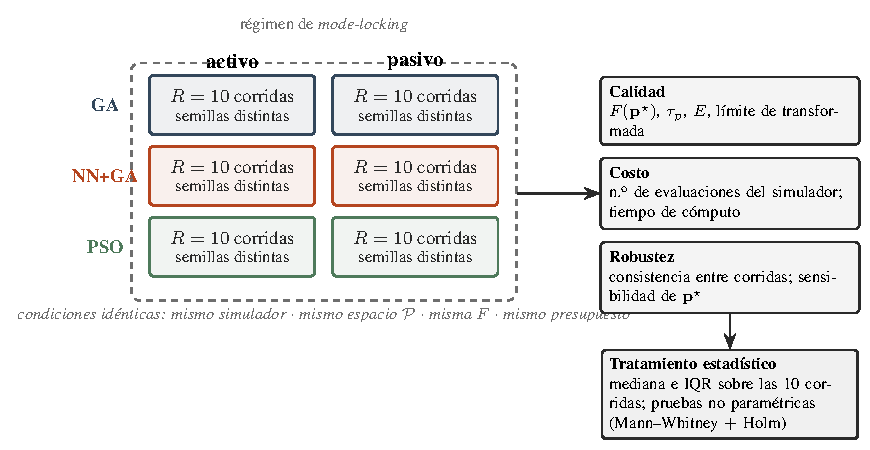
\includegraphics[width=\textwidth]{chapters/images/ch4/fig_matriz_experimental.pdf}
    \caption[Diseño experimental y protocolo comparativo]{Diseño experimental. La
    matriz enfrenta las tres estrategias (filas) en los dos regímenes de
    \emph{mode-locking} (columnas); cada celda se ejecuta $R=10$ veces con semillas
    distintas para tratar la naturaleza estocástica de los métodos. Sobre un fondo
    de condiciones idénticas (mismo simulador, mismo espacio $\mathcal{P}$, misma
    función de mérito y mismo presupuesto), la única variable que cambia es el
    algoritmo. El desempeño se juzga con tres familias de métricas (calidad, costo
    y robustez) y las diferencias se contrastan con pruebas no paramétricas
    (Mann--Whitney con corrección de Holm) sobre la mediana de las repeticiones.}
    \label{fig:matriz-experimental}
\end{figure}

\subsection{Control de la aleatoriedad, repeticiones y tratamiento estadístico}
\label{sec:aleatoriedad}

Las tres estrategias son \emph{estocásticas}: su resultado depende de la
inicialización aleatoria y de las decisiones al azar que toman durante la búsqueda.
Una única ejecución de cada método sería, por tanto, una muestra poco informativa y
potencialmente engañosa. Para obtener conclusiones fiables, cada combinación de
algoritmo y régimen se ejecuta \emph{múltiples veces de forma independiente},
variando únicamente la semilla del generador de números aleatorios, que se registra
en cada corrida para garantizar que los experimentos puedan repetirse. El desempeño
no se reporta como un único número, sino como una \emph{distribución} sobre las
repeticiones (resumida por su mediana y su dispersión), y las diferencias entre
métodos se contrastan con las herramientas estadísticas apropiadas, en lugar de
compararse sobre corridas aisladas. Controlar así la aleatoriedad y las repeticiones
es lo que permite atribuir los resultados a la metodología y no a las
particularidades de una ejecución concreta, un requisito de fiabilidad bien
establecido en el aprendizaje automático aplicado \cite{Pineau2021}. En concreto, cada
celda se repite diez veces con semillas derivadas de una semilla maestra, y las
diferencias de $F^\ast$ se contrastan con la prueba $U$ de Mann--Whitney bilateral,
con corrección de Holm dentro de cada régimen.

% [REV-2026-11-17] subsección nueva: el piloto (wiki/log.md 2026-07-22; configs/experiments/matrix_prod_v1.yaml)
\subsection{Calibración piloto}
\label{sec:calibracion_piloto}

Antes de la producción se ejecutó una matriz piloto con la misma configuración, dos
repeticiones por celda y un presupuesto de cien evaluaciones. El piloto cumplió dos
funciones. La primera fue medir el costo: unos $2.2$~s por evaluación en promedio,
algo más en el régimen activo. Con esa cifra se fijaron el presupuesto de $400$
evaluaciones por corrida y las diez repeticiones por celda, unas once horas de cómputo
en serie. La segunda fue detectar un mérito mal equilibrado: con $E_{\mathrm{ref}}=4$~nJ,
el término de energía dominaba al de duración en un factor cercano a seis, y en el
régimen activo el GA alcanzaba el mayor mérito con pulsos de unos $160$~ps. El objetivo
efectivo ignoraba la duración. Se fijó entonces $E_{\mathrm{ref}}=40$~nJ, del orden de la
energía máxima alcanzable en la caja, de modo que ambos términos quedaran en el mismo
orden. La configuración resultante se congeló antes de la producción y es la que recoge
la Tabla~\ref{tab:parametros_estudio}.

\subsection{Reproducibilidad y herramientas de implementación}
\label{sec:reproducibilidad}

El estudio se articula como un protocolo comparativo \emph{reproducible}, lo que
exige registrar y versionar todos los elementos de los que dependen los resultados.
% [REV-2026-11-17] herramientas nombradas (antes genéricas)
Todo el código se escribió en Python. El simulador y los algoritmos GA y PSO se
implementaron desde cero con NumPy y SciPy, sin bibliotecas de optimización, porque
los algoritmos son el objeto del estudio y debían contar exactamente las evaluaciones
del simulador; la red sustituta se implementó con PyTorch. La producción se ejecutó en
un portátil bajo WSL (Ubuntu, Python 3.12.3, NumPy 2.5.1, SciPy 1.18.0, PyTorch 2.13.0),
y cada corrida registra su semilla, las versiones del software y la configuración
completa. La implementación se verifica con un conjunto de $68$ pruebas automáticas
(pytest) que incluye las del simulador de la Sección~\ref{sec:sim_verificacion}. Se consignan, en segundo
lugar, los \emph{valores concretos} de todos los parámetros del estudio, los rangos
físicos de las variables de decisión (Sección~\ref{sec:restricciones}), los pesos
$w_i$ y la penalización $\Pi$ de la función de mérito
(Sección~\ref{sec:funcion_merito_op}), los hiperparámetros de cada algoritmo
(Secciones~\ref{sec:ga_hiperparametros}, \ref{sec:nnga_entrenamiento}
y~\ref{sec:pso_hiperparametros}), y los parámetros de la discretización numérica
$N$, la ventana temporal y el número de vueltas (Sección~\ref{sec:sim_integracion}),
que se reúnen en una tabla única y se mantienen idénticos para los tres métodos en lo
que no es propio de cada algoritmo.

% Tabla generada automáticamente desde la configuración versionada del código
% (scripts/make_table_4_6_4.py). NO editar a mano: regenerar tras cualquier cambio.
% Tabla ch4 §4.6.4 — GENERADA por scripts/make_table_4_6_4.py
% desde matrix_prod_v1.yaml y sus configs. NO editar a mano:
% regenerar tras cualquier cambio de configuración.
\begin{table}[htbp]
  \centering\small
  \caption{Parámetros del estudio comparativo (generados desde la
  configuración versionada del código; véase la Sección~\ref{sec:reproducibilidad}).}
  \label{tab:parametros_estudio}
  \begin{tabular}{ll}
    \hline\multicolumn{2}{c}{\textbf{Cavidad fija (ambos regímenes)}}\\\hline
    $l$ & 0.1 \\
    $\Omega_g$ & $2\pi\times60$~GHz \\
    $T_R$ & 4~ns \\
    $E_{\mathrm{sat},L}$ & 4.5~nJ \\
    $\omega_m$ & $2\pi\times250$~MHz \\
    \hline\multicolumn{2}{c}{\textbf{Discretización y estacionario}}\\\hline
    $N$ & 2048 \\
    ventana temporal & 1.024~ns \\
    vueltas máx. & 50000 \\
    tolerancia (bloques de 100) & 1e-06 \\
    semilla inicial & gaussiana 68~ps, 4~nJ \\
    \hline\multicolumn{2}{c}{\textbf{Rangos: régimen activo $\mathbf{p}=(g_0,D,\delta,M)$}}\\\hline
    $g_0$ & $[0.15,\ 1.5]$ \\
    $D$ & $[-30,\ 30]$~ps$^2$ \\
    $\delta$ & $[0,\ 5]$$\times10^{-4}$~W$^{-1}$ \\
    $M$ & $[0.01,\ 0.5]$ \\
    \hline\multicolumn{2}{c}{\textbf{Rangos: régimen pasivo $\mathbf{p}=(g_0,D,\delta,q_0,\gamma)$}}\\\hline
    $g_0$ & $[0.15,\ 1.5]$ \\
    $D$ & $[-30,\ 30]$~ps$^2$ \\
    $\delta$ & $[0,\ 5]$$\times10^{-4}$~W$^{-1}$ \\
    $q_0$ & $[0.01,\ 0.3]$ \\
    $\gamma$ & $[0.1,\ 10]$$\times10^{-4}$~W$^{-1}$ \\
    \hline\multicolumn{2}{c}{\textbf{Función de mérito}}\\\hline
    $(w_\tau, w_E, w_\sigma)$ & (1, 0.5, 0.5) \\
    $(\tau_{\mathrm{ref}}, E_{\mathrm{ref}}, \sigma_{\mathrm{ref}})$ & (10~ps, 40~nJ, 0.001) \\
    penalización $(\Pi_0, \Pi_1)$ & (10, 10) \\
    \hline\multicolumn{2}{c}{\textbf{GA (idéntico dentro de NN+GA)}}\\\hline
    población / élite / torneo & 20 / 2 / 3 \\
    $p_c$ / $p_m$ / escala mut. & 0.9 / 0.15 / 0.1 \\
    \hline\multicolumn{2}{c}{\textbf{PSO}}\\\hline
    enjambre / $\omega$ / $c_1,c_2$ & 20 / 0.9$\to$0.4 / 1.5, 1.5 \\
    $v_{\max}$ / frontera & 0.2$\times$rango / recorte$+v{=}0$ \\
    \hline\multicolumn{2}{c}{\textbf{NN+GA (sustituto MLP)}}\\\hline
    LHS inicial / ciclos / verif. & 40 / 6 / 5 \\
    capas ocultas / lr / lote & (64, 64) / 0.001 / 32 \\
    \hline\multicolumn{2}{c}{\textbf{Protocolo}}\\\hline
    presupuesto por corrida & 400 evaluaciones \\
    repeticiones por celda & 10 \\
    semilla maestra & 20260722 \\
    \hline
  \end{tabular}
\end{table}


Se adopta, por último, una \emph{cadena de procedencia} explícita que liga cada
resultado del capítulo siguiente con los elementos que lo generaron: cada figura se
remite al script que la produce (con su versión), al conjunto de datos que consume,
a la configuración con que se generó y a su documentación. Esta trazabilidad
completa (de la figura al script, al dataset y a su configuración) es lo que
convierte al protocolo en algo repetible por un tercero y no en una descripción
aproximada.

Conviene reconocer, para cerrar, el límite que esta reproducibilidad no elimina.
Como el estudio emplea simulación pura como generador de datos, sus conclusiones se
circunscriben al modelo de la ecuación maestra y a los rangos de parámetros
explorados, y no incorporan de forma plena el ruido, la deriva y las no idealidades
de un montaje real, la brecha \emph{sim\-/to\-/real} que la propia formulación del
alcance reconoce (Sección~\ref{sec:hipotesis-alcance}), \cite{Zhao2020}. El protocolo
garantiza que los resultados sean reproducibles \emph{dentro} de ese modelo; su
extrapolación al laboratorio queda fuera del foco del estudio y se retoma como
horizonte en la discusión.


% ============================================================
%  Seccion 4.7 -- Sintesis de la metodologia (cierre)
% ============================================================

\section{Síntesis de la metodología}
\label{sec:sintesis_metodologia}

Este capítulo ha traducido la pregunta de investigación en un experimento concreto y
ejecutable. Partiendo de la ecuación maestra de Haus, ha construido un simulador de
la cavidad que reproduce los regímenes de operación conocidos y se verifica contra
las soluciones analíticas disponibles (Sección~\ref{sec:modelo_numerico}); sobre él
ha planteado un problema de optimización bien definido, un vector de decisión acotado
por rangos físicos y por la restricción de estabilidad frente al \emph{Q\-/switching},
y una función de mérito escalar construida sobre los observables del pulso
(Sección~\ref{sec:formulacion_problema}),; ha especificado la implementación de las
tres estrategias que lo resuelven, el algoritmo genético como línea base
(Sección~\ref{sec:ga_impl}), la red neuronal sustituta acoplada al algoritmo genético
(Sección~\ref{sec:nnga_impl}) y la optimización por enjambre de partículas
(Sección~\ref{sec:pso_impl}),; y ha fijado el protocolo con que se comparan
(Sección~\ref{sec:diseno_experimental}).

Tres decisiones de método vertebran ese diseño y conviene retenerlas. La primera es
que las tres estrategias comparten el paradigma de la optimización global sin
derivadas y difieren solo en la mecánica de búsqueda (la recombinación evolutiva, el
sustituto aprendido o el movimiento del enjambre), lo que las hace verdaderamente
contrastables. La segunda es que todo lo que no es el algoritmo permanece fijo: el
mismo simulador, el mismo espacio de parámetros, la misma función de mérito y el
mismo presupuesto de evaluaciones, sobre los dos regímenes de bloqueo de modos. La
tercera es que el desempeño no se juzga por una corrida aislada, sino por una batería
de repeticiones controladas y por tres familias de métricas (calidad del pulso, costo
computacional y robustez) tratadas estadísticamente. Es la conjunción de estas tres
decisiones la que responde de manera directa a las dos brechas que motivan la tesis:
la de \emph{objeto}, al cubrir el régimen activo junto al pasivo, y la de
\emph{método}, al sustituir la colección de estudios de caso por un benchmarking
controlado y reproducible (Sección~\ref{sec:aporte}).

Con la metodología así definida, el estudio queda listo para su ejecución. El
capítulo de resultados aplica este protocolo a la matriz de experimentos (los tres
optimizadores sobre los dos regímenes) y reporta, bajo las métricas comunes, el
desempeño comparado de cada estrategia; su discusión interpretará esas diferencias a
la luz de la física de la cavidad y de la hipótesis de trabajo
(Sección~\ref{sec:hipotesis-alcance}), y delimitará el alcance de las conclusiones
frente a la brecha entre la simulación y el laboratorio.
